\documentclass[WHATMANUAL.tex]{subfiles}

\begin{document}

\chapter{Gapless weather data series creation}\label{chap:gapfilling}

\section{Downloading and formatting data from the CDCD}

The Canadian Daily Climate Database (CDCD) contains daily air temperature and precipitation from 1840 to the present for about 8450 stations distributed across Canada. Data can be downloaded manually on the Government of Canada website as CSV files on a yearly basis, or it is possible to acquire the entire database by ordering a DVD. The former option involves a lot of repetitive manipulations and can become quickly a time consuming task while the latter does not offer a convenient way to update the data. Moreover, the organization of the downloaded CDCD data files in a more convenient format can also represent a tedious task when done manually.

WHAT alleviates this process by providing a graphical interface to the online CDCD database that allows to query stations interactively by location coordinates, download the available data, and automatically rearranged the data in a format compatible with WHAT. All of these features are available from the tab \emph{Download Data} shown in Figure~\ref{fig:tab_dwnldData}.

\begin{figure}[!ht]
\centering
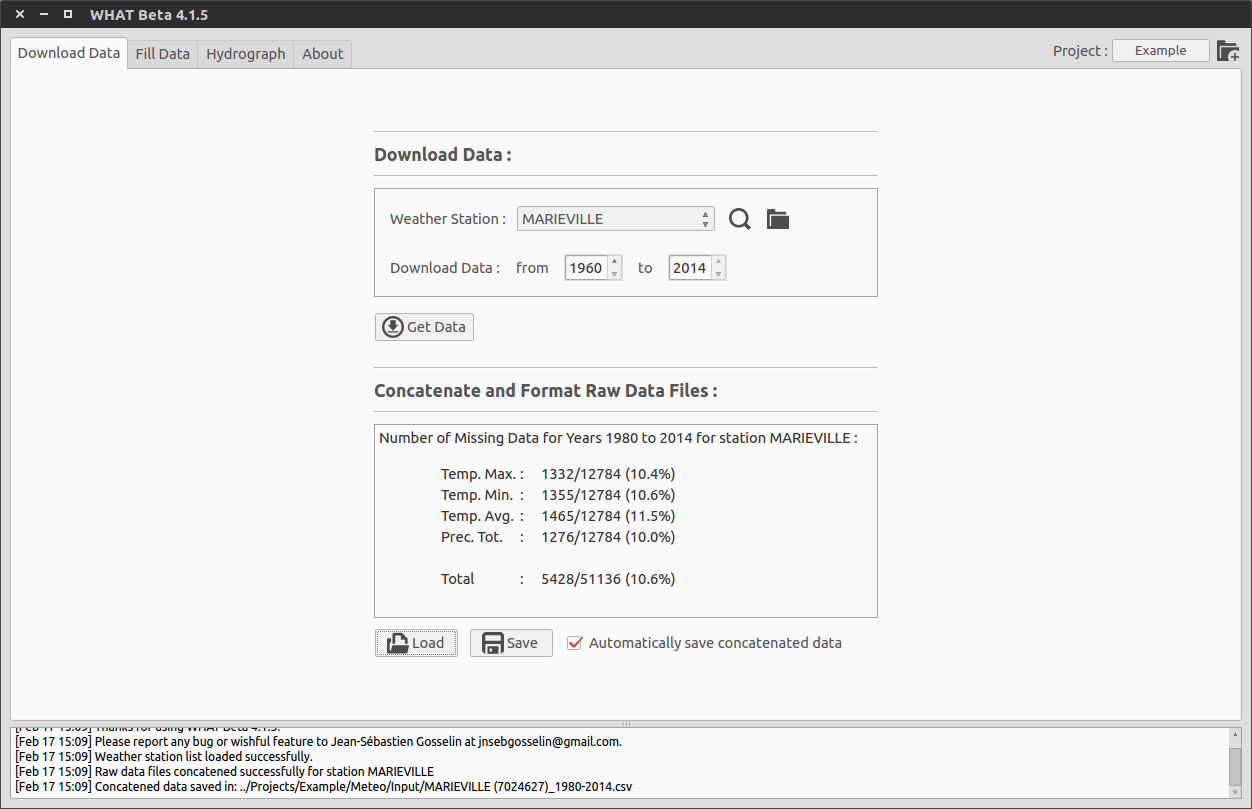
\includegraphics[width=0.75\textwidth]{img/WHAT_Screenshot000}
\caption[Tab ``Download Data''.]{Tab ``Download Data''.}
\label{fig:tab_dwnldData}
\end{figure}

\subsection{Searching for Stations}

To start searching for stations in the online CDCD, go in the tab \emph{Download Data} and click on the small magnifying glass icon located next to the \emph{Weather Station} drop down list, that should be empty if you have just created a new project. This will open a new dialog window (see Figure~\ref{fig:Screenshot_search4stations}) where you can search for stations located within a given radius around a location defined in latitude and longitute decimal degrees. It is possible to further narrow down the search by including only stations that have data within a given period. 

Clicking on the button \emph{Search} initiates the search for weather stations with the specified parameters. The results are saved in the file ```weather\_stations.lst'' and the \emph{Weather Station} drop down list is updated to list all the stations found during the search.

\begin{figure}[!ht]
\centering
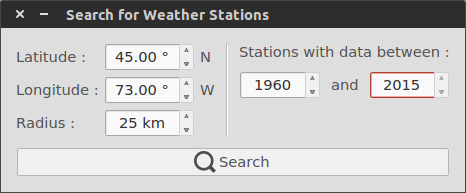
\includegraphics[width=0.5\textwidth]{img/WHAT_Screenshot_search4stations}
\caption[Graphical interface to the online CDCD database.]{Graphical interface to the online CDCD database.}
\label{fig:Screenshot_search4stations}
\end{figure}

Alternately, it is possible to use a custom list of Canadian stations generated manually without using the graphical interface. This is done by retrieving station information from their unique url directly on the government of Canada website (\url{www.climate.weather.gc.ca}). The information must be saved in a TSV text file with the ``.lst'' extension. The list can be loaded in WHAT by clicking on the small folder icon located next to the \emph{Weather Station} drop down list. A detailed example is presented for the weather station Marieville, located in southern Quebec, in Appendix~\ref{app:custom_station_list}.

\subsection{Downloading Data}

Once a list of weather station has been generated in WHAT, either by an automatic search with the interface or by opening a custom weather station list, data can be downloaded from the online CDCD by selecting the desired station in the drop-down menu list and clicking on the button \emph{Get Data}. For each year between the values specified in the \emph{Download Data} year range, WHAT will automatically download the weather data from the CDCD and save the results as a CSV file in the \emph{Raw} folder (see section~\ref{subsec:folder_structure} for each year individually).

The downloading process can be stopped at any time by clicking on the button \emph{Get Data} which will then be displaying a red stop icon. Before downloading data for a given year, WHAT will first check if data already exist for that whole year in the folder \emph{Raw}. If it is the case, data for this year won't be downloaded and the process will pass to the following year, otherwise data will be downloaded and saved normally from the CDCD. Detailed information about the program transactions during the downloading process are printed in the console area located at the bottom of the interface (see section~\ref{sec:GUI_overview}).

\subsection{Formatting Data}

As soon as a downloading task ends successfully for a given weather stations, WHAT automatically format and concatenate the data. That is data for each year are put together end to end in chronological order and only data related to air temperature (mean, max and min) and total precipitation are kept. In addition, NaN values will be put everywhere data are missing. Finally, statistics about the missing values in the dataset for each meteorological variable will be displayed in the \emph{Concatenate and Format Raw Data Files} section.

By default, WHAT will automatically save the formatted data series in a single TSV file within the folder \emph{Input} (see section~\ref{subsec:folder_structure}. You can save any other copy of the formatted data set anywhere on your computer by clicking on the button \emph{Save}. The automatic saving of formatted data series can be disabled by unchecking the \emph{Automatically save concatenated data} option. 

It is also possible to open previously downloaded weather data files in WHAT by clicking on the button \emph{Load} and selecting the desired files in the dialog window. WHAT will then automatically format and concatenate the data and a new concatenated data files and save the results automatically if the \emph{Automatically save concatenated data} option is checked. Alternatively, the formatted data series can be saved by clicking on the button \emph{Save}.

\section{Gap filling daily weather records}\label{guide-gapfilling}

One of WHAT main utility is the automatic gap filling of daily weather data records. This feature is accessible from the tab \emph{Fill Data} shown in Figure~\ref{fig:tab_fillData}. On start-up or after opening a project, WHAT automatically scans the content of the \emph{Input} folder for valid weather data files and displays the result as a list of weather station names under the label \emph{Fill Data for Weather Station}. The list of stations won't be refreshed automatically if new data files are added to the Input folder after the project has been opened. The button \emph{Refresh} located next to the list of stations can be used for this purpose. In addition, each time WHAT search the Input folder for valid weather data files, it automatically computes statistics about the period over which data are available for each station and the number of missing data in the weather time-series and saves the results in the file named ``weather\_datasets\_summary.log'' (see section~\ref{subsec:folder_structure}).

\begin{figure}[!ht]
\centering
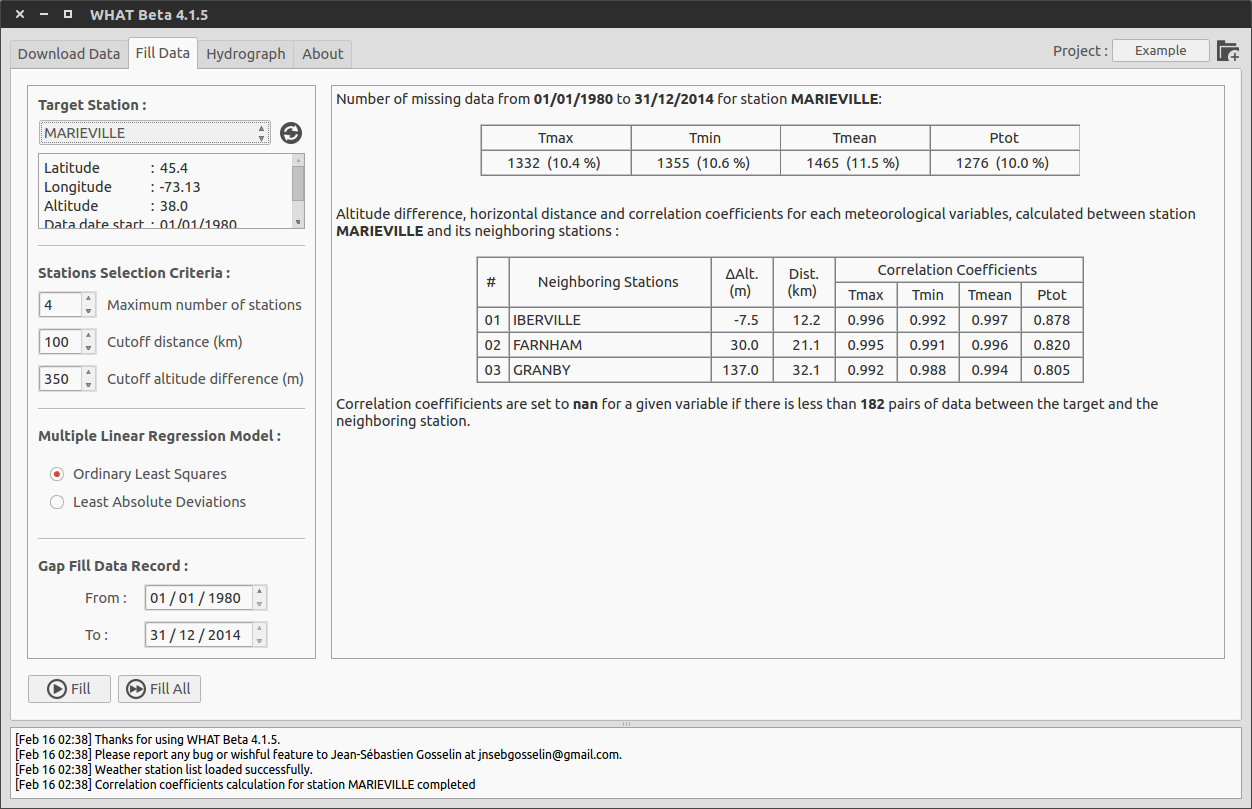
\includegraphics[width=0.75\textwidth]{img/WHAT_Screenshot001}
\caption[Tab ``Fill Data''.]{Tab ``Fill Data''.}
\label{fig:tab_fillData}
\end{figure}

If the Input folder is not empty, selecting a station from the drop-down list will automatically initiate the computation of correlation coefficients between the data of the selected station and all of the remaining stations (herein called the neighboring stations), as well as horizontal distances and elevation differences. In addition, information about the number of missing values in the data of the selected weather station are also computed. The results are displayed in the view panel located on the right side of the interface. Correlation coefficients that fall below a value of 0.7 are displayed in red in the table. This is only meant as guidance for the user and has no impact on the gap filling procedure.

The process to fill the gaps in the data of the selected weather station can be launched by clicking the button \emph{Fill} located at the bottom of the left side panel of the interface. Each missing value is estimated with a multiple linear regression (MLR) model generated with the synchronous weather time series of the selected and neighboring stations. The routine uses the data from the neighboring stations that are best correlated with the data of the selected station, up to the maximum number of stations defined by the user. For example, in Figure~\ref{fig:tab_fillData}, the program would use the neighboring stations with the best correlation coefficient values up to a maximum of 4 stations. If for a given date all the neighboring stations have missing data synchronously with the selected station, a NaN value is kept in the dataset at this particular time.  

It has been demonstrated that the MLR method outperforms most of the commonly used techniques for the estimation of missing data in daily meteorological records \citep{eischeid_quality_1995,eischeid_creating_2000,xia_forest_1999}. The user can also choose between an Ordinary Least Squares (OLS) or a Least Absolute Deviations (LAD) criterion for the generation of the MLR model. The LAD criteria is more robust to outliers than the OLS but is more demanding in computation time. 

In addition, data correlation between two stations for a given meteorological variable will generally decreases as difference in altitude and distance increase. Therefore, it is possible to specify a cutoff distance and a cutoff altitude difference for which neighboring stations that fall above these cutoff values are excluded from the gap filling procedure. A value of 100~km for the cutoff distance and 350~m for the cutoff altitude difference are set as default values in the program, based on the literature 
\citep{tronci_comparison_1986,xia_forest_1999,simolo_improving_2010}. 

WHAT will fill the gaps in the data between the dates specified by the user and automatically save the gapless daily weather time series in a tab-separated values (TSV) text file with the extension ``.out'' within the sub-folder \emph{Output} of the folder \emph{Meteo} (see section~\ref{subsec:folder_structure}). The file is named after the weather station name and its unique IDN. For example, the resulting output file for the station named Marieville in Figure~\ref{fig:tab_fillData} would be ``MARIEVILLE (7024627)\_1980-2014.log''. In addition, detailed information about every missing value estimated by WHAT to fill the gap in the data are saved in a file with the same name as the ``.out"" file but with a ``.log'' extension.

It is also possible to fill the gaps in the data for all the stations in batch by clicking on the button \emph{Fill All}. The parameters for the gap filling process will then be kept the same for all the stations.

Finally, it is possible to assess the incertitude of the method used to estimate the missing values with a jackknife procedure. This is an advanced feature that is in experimental states and thus cannot presently be activated directly from the GUI. The activation of this feature must be done by changing the value of the field ``Full Error Analysis'' from 0 to 1 in the file named ``WHAT.pref'' that is located within the folder named ``WHAT'' (see Section~\ref{sec:intallation}). A software restart is required for this change to take effect. This feature is discussed in more details in Section~\ref{chap:Missing_weather_theory}. Activating this feature will have a very strong impact on the performance of the gap filling procedure, especially if the least absolute deviation regression model is selected.

\section{Using weather data from other sources}

Presently, it is not possible to automatically download and format data of weather stations located in the U.S. or in any other country than Canada. This feature may be added for the U.S. in a future release of the software.

However, it is still possible to use weather data from any sources in WHAT either for filling the gaps in the time-series or for the interpretation of water-level time-series, as long as the data are saved in a format compatible with WHAT.

It is strongly recommended to use a copy of one of the sample files that are provided in the project example that is distributed with the software and fill the information and the data directly in them. The files must be kept in a tab-separated values text format either with the extension ``.csv'' or ``.out''. This can be achieved in any standard spreadsheet application such as Microsoft Excel or LibreOffice Calc. The format of the header must be observed faithfully in those files. In addition, NaN values must be entered where data are missing. Data must also be in chronological order, but do not need to be continuous over time. That is missing blocks of data (e.g., several months or years) can be completely omitted in the time-series. These missing blocks of data will be estimated and filled during the gap filling procedure or will be ignored for the plotting of the hydrograph.

\end{document}